%****************************************************************************
%** Copyright 2002 by Lukas Ruf, ruf@topsy.net
%** Information is provided under the terms of the
%** GNU Free Documentation License http://www.gnu.org/copyleft/fdl.html
%** Fairness: Cite the source of information, visit http://www.topsy.net
%****************************************************************************
%****************************************************************************
%** Last Modification: 2005-07-11 1600
%** 2005-07-11	Bernhard Tellenbach
%**							This is an addapted version of the Introduction.tex file
%**							Added table example (footnotes,multicolumn)
%**							Examples for different text sizes
%**							Updated eps file inclusion example for use with graphicx pkt. 
%****************************************************************************

\chapter{\label{chapter2}Background}

In this chapter, we give a brief overview of BGP in \ref{chapter2:BGP} and explain the problem of long convergence time upon remote failure in BGP. We highlight the architecture and key insights of both iSDX and Swift in \ref{chapter2:iSDX} and \ref{chapter2:Swift}, respectively. The architecture of both frameworks are very similar, they are based on an SDN switch, an SDN controller and a route server. In the next chapter, we explain how these similarities can be put to use in the implementation.

\section{\label{chapter2:BGP}BGP}

\rb{also talk about the attributes of the announcements (prefix, AS path). That way you can later explain that thanks to these attributes, you can make assumptions about the failures. If the AS path was not present, you couldn't say anything about the remote failure.}

The Border Gateway Protocol (BGP) allows autonomous systems to exchange routing information with each other. The routing information is communicated on a per prefix basis using BGP updates. BGP updates contain the prefix and the AS-path the packet will traverse, if packets are sent via this route. There are two types of updates, announcements and withdraws. Announcements inform that the prefix can be reached via this route and withdraws inform that the previously announced prefix cannot be reached via this route anymore. 

Upon receiving a BGP update routers compute the best route to the prefix of the update and then send updates to their peers. Routers only send announcements with their own best route to the prefix and if the routers do not know a route to the prefix they send withdraws.

Convergence time in BGP upon remote failure can be slow.
This is because of the way updates propagate trough the network. Changes are only passed on once routers have finished computing the best route to the prefix. Only once all the best path computation has finished, a router is able to make sure that packets do no get sent into a black hole or loop anymore.



\section{\label{chapter2:iSDX}iSDX}

The iSDX is an internet exchange point enhanced with an SDN switch and SDN controller.
An internet exchange point is a physical location where multiple autonomous systems meet to exchange traffic and BGP routes. \rb{An exchange point provides a fabric for the networks to interconnect. Each network attaches with one or multiple routers to this fabric. To reduce the burden on the network operators, internet exchange points often provide a route server. Thanks to the route server, each border router only has to peer with the route server instead of all other route servers while still receiving the announcements of all other IXP participants. However, even though many different routes might be available for a single prefix, participants of a traditional IXP can only use a single route per prefix.} 

The iSDX allows its participants to not only make use of this additional routes, but also gives the participants  more fine-grained control over the routing decisions. A Participant connects to the iSDX as if it were a traditional IXP and is able to specify special policies that allow to use multiple routes at once and control routing beyond the prefix.

\rb{you can omit the "will": e.g., we show instead of we will show}
We first show the iSDX architecture in \ref{chapter2:iSDX:iSDX_architecture}, explain the different policies and their capabilities in \ref{chapter2:iSDX:policies} and how the iSDX features are implemented using a virtual next-hop and repurposing the destination mac address in \ref{chapter2:iSDX:VNH_VMAC}.

\subsection{\label{chapter2:iSDX:iSDX_architecture}iSDX Architecture}
\begin{figure}[h]
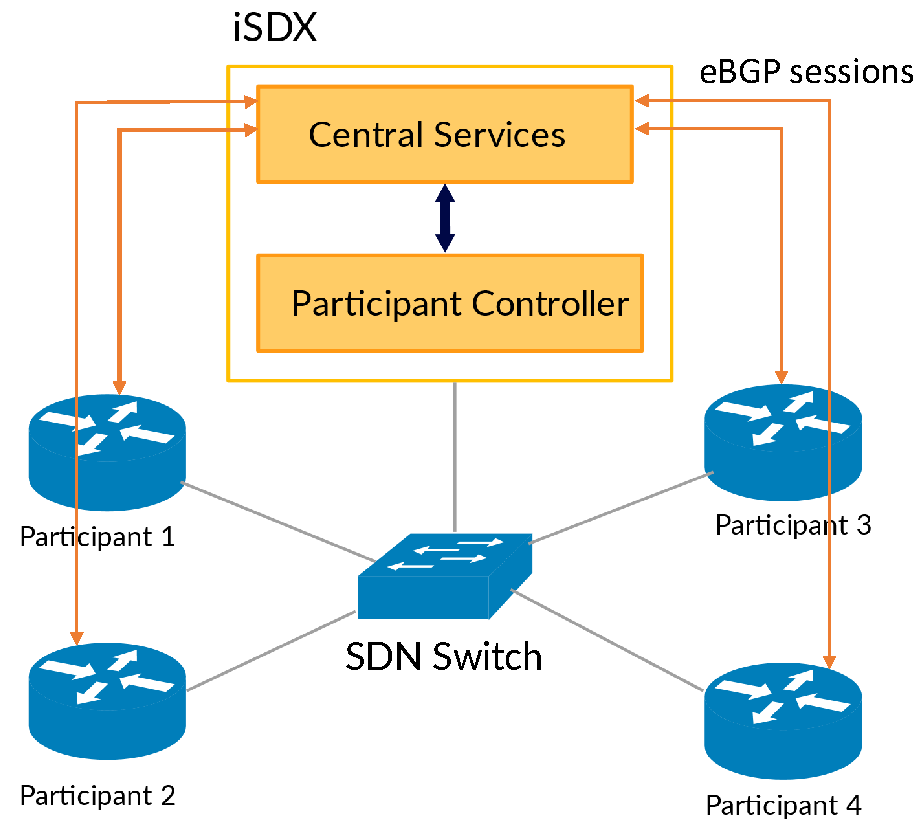
\includegraphics[scale = 0.4]{Figures/isdx_architecture_cropped.pdf}
\caption{iSDX architecture}
\end{figure}

The iSDX architecture consists of two main parts: \emph{(i)} the Central Services and \emph{(ii)} the Participant Controller.

The Central Services has two tasks. \emph{(i)} It collects all BGP updates and ARP queries centrally and forwards them to the corresponding participant controller. \emph{(ii)} It makes sure that BGP connection, default forwarding and ARP traffic is correctly handled by installing flow rules.

Every participant has its own participant controller. This allows each participant to make its own best path decision. The participant controller receives and processes BGP updates from the central route server. Every participant controller has a local routing information base, which keeps track of all the received routes, currently used routes and routes advertised to other participants. It takes care of the virtual next-hop and VMAC assignment. It handles ARP requests and sends out gratuitous ARP replies. Before BGP updates get sent to the participants border router they are processed by the participant controller. Also, it installs all the flow rules which are necessary for its policies to be enforced.

\subsection{\label{chapter2:iSDX:policies}Policies}
\rb{Policies allow a participant to specify forwarding behavior which deviates from the default best path forwarding. They can be specified on any part of the header.}
Policies match on a field of the packet header and then forward the packet to a participant. Policies are implemented as flow rules that the participants controller programs into the SDN switch. Two types of policies exist: \emph{(i)} outbound policies that handle all out-going traffic and \emph{(ii)} inbound policies that handle all incoming traffic.

\paragraph{\label{chapter2:iSDX:policies:outbound policies}Outbound Policies:}
Outbound policies let participants direct packets going from themselves to the iSDX. They allow the participants forward packets onto another path than the best path. An example of an outbound policy is shown in Figure~\ref{fig:isdx_policies}, where participant \emph{A} has defined two outbound policies directing traffic away from the best path to either one of the other two participants. \rb{change the figure to include a identifier for each policy such that you can write: Has defined two outbound policies (X and Y)...}

\paragraph{\label{chapter2:iSDX:policies:inbound policies}Inbound Policies:}
Inbound policies allow participants to specify how incoming packets are handled. In effect they allow the participant to choose to which of his own routers packets from the iSDX get sent to. An example of an inbound policy is shown in Figure~\ref{fig:isdx_policies}, where participant C has defined two inbound policies directing traffic to either one of it's routers depending on the destination port. 

\begin{figure}[h]
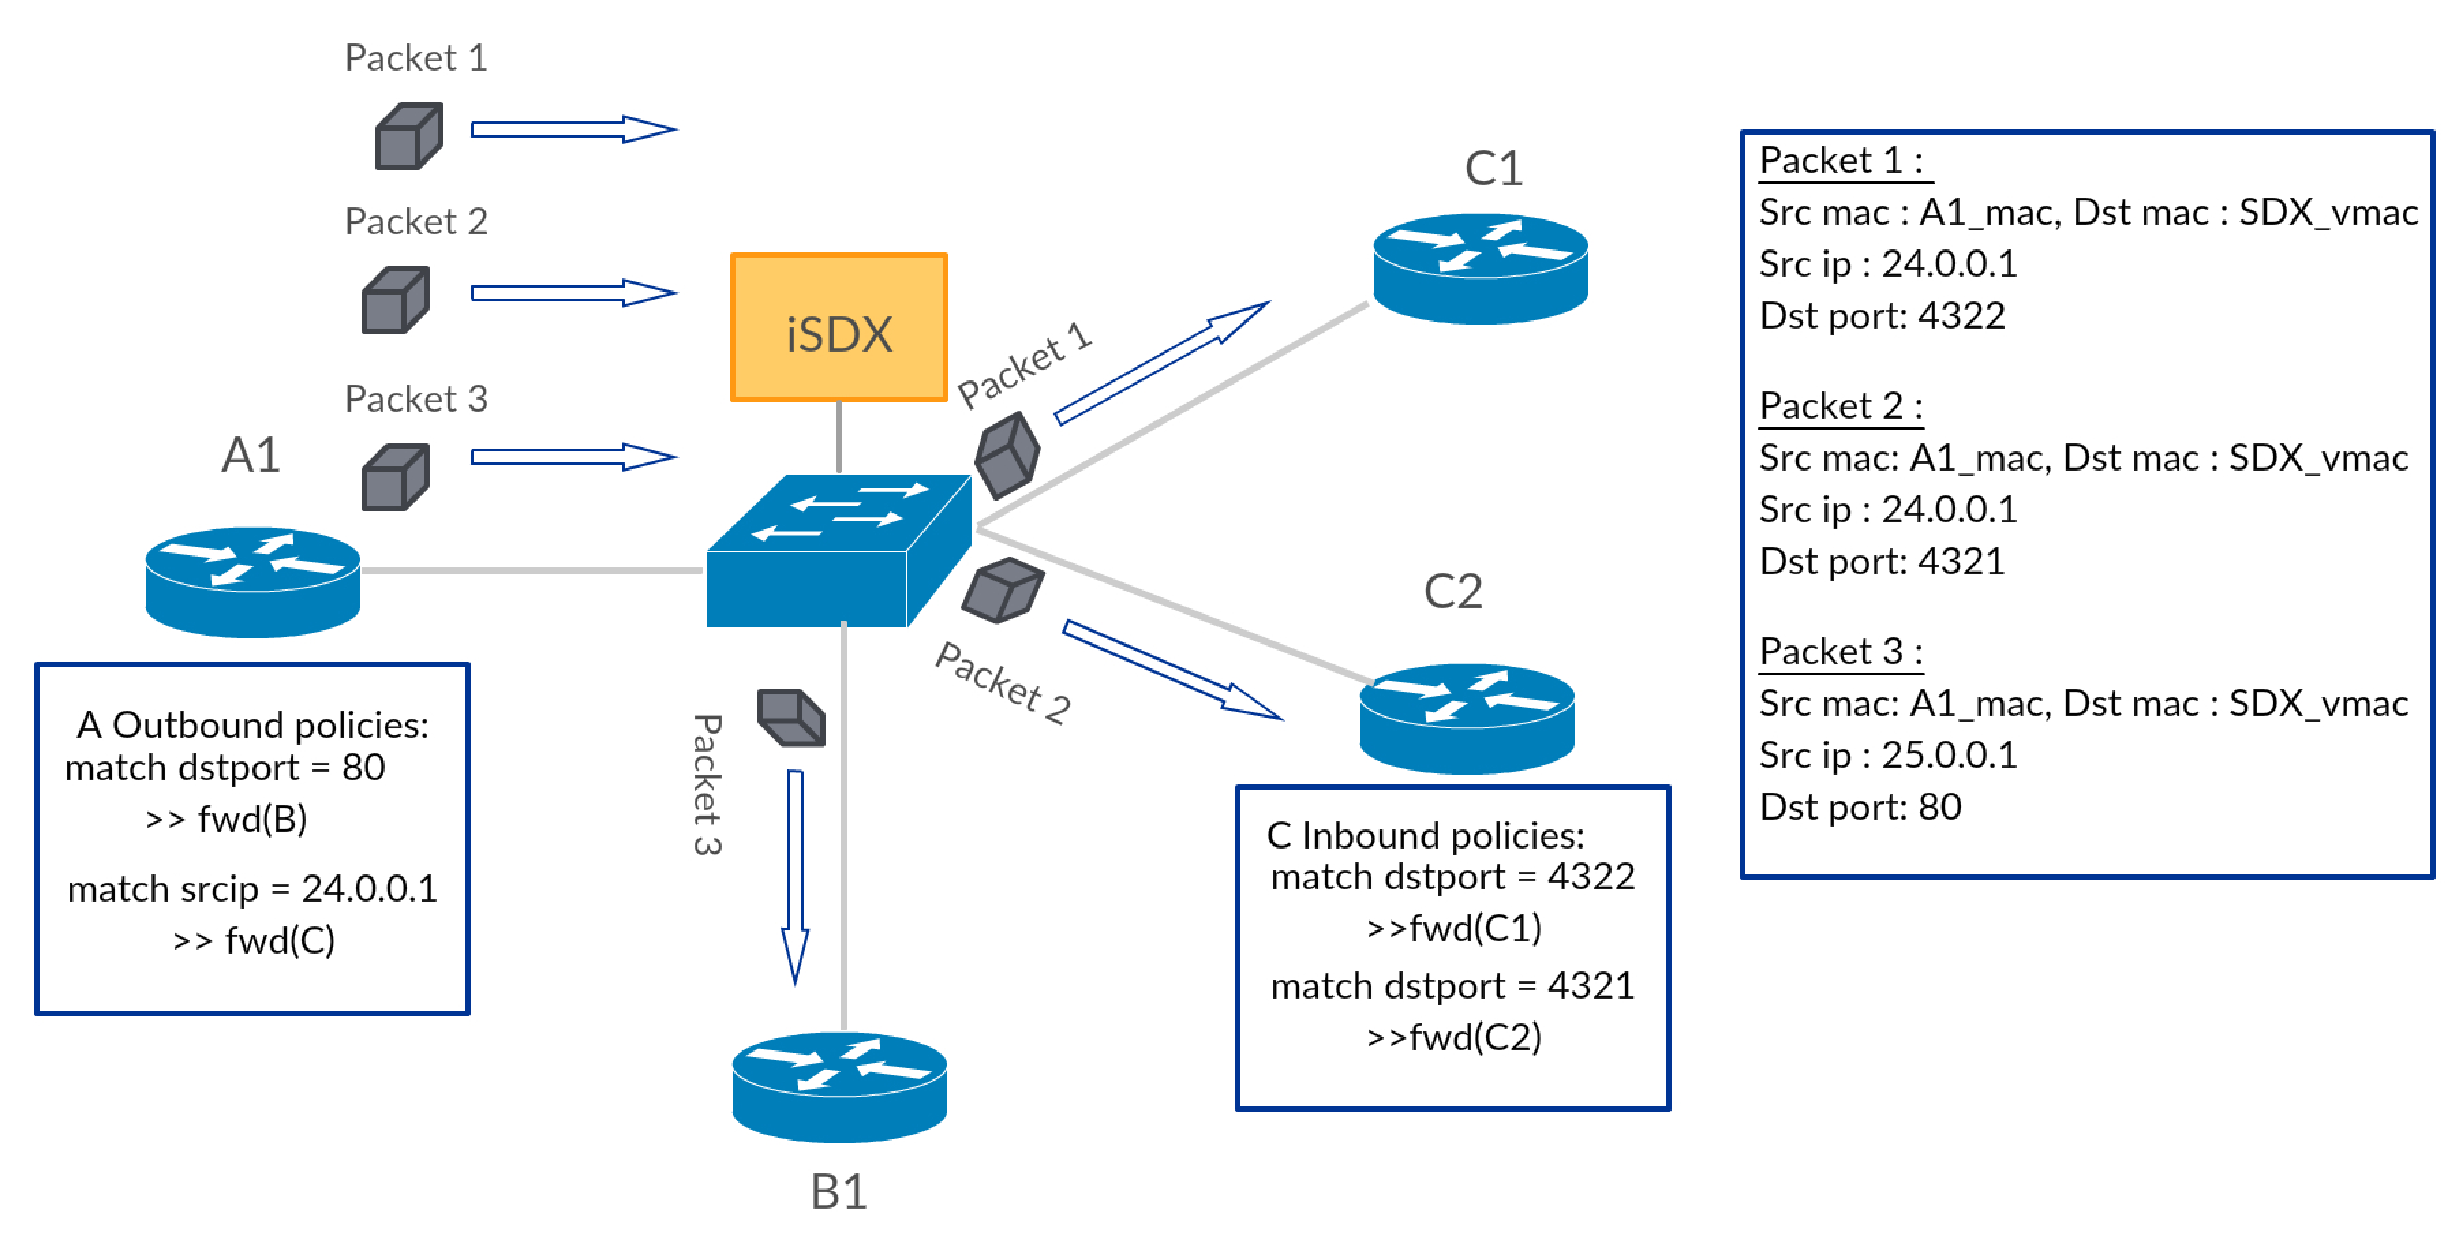
\includegraphics[scale = 0.32]{Figures/bckgrnd_sdx_policies.pdf}
\caption{Example of outbound and inbound policies at an iSDX connected to three participants}
\label{fig:isdx_policies}
\end{figure}
  

\subsection{\label{chapter2:iSDX:VNH_VMAC}Virtual Next-Hop, Virtual MAC Address}

\rb{better explain why they should be restricted. First, write why they should be restricted. Then write that it is not practical to restrict them as the routing might change very often and then they would always have to adapt their policies and then write, that the iSDX does not restrict them and takes care of this. Along the lines of what I restructured below. Just needs some polishing.}

Note that when specifying a policy, the network operator does not have to take into account whether the specified destination actually is able to handle that traffic. Some policies might direct packets to participants that did not advertise the prefix to that participant or simply do not know a route to the prefix. Participants are not restricted when defining outbound policies. This is a problem because outbound policies can end up violating BGP advertisements. It is not possible to require participants to only specify feasible policies as the routing information is quite volatile and network operators would constantly need to update their policies to make sure none of the traffic is blackholed. 

The iSDX solves this problem by attaching additional information to each packet. This additional information is embedded into the destination mac address, transforming the destination mac addresses of packets traversing the SDN switch into a Virtual Mac Address (VMAC).
In the VMAC the participant controller encodes the participants advertising the prefix of the packet and the BGP best next hop participant for this prefix. The first part is used every time a outbound policy is applied. The outbound policy checks if the participant the outbound policy is sending packets to has advertised the prefix. The second part is used if the packet does not match any outbound policy. Default rules in the SDN switch match on the best next-hop participant and send the packet to this participant.

Each border router replaces the destination MAC address with the corresponding VMAC before sending a packet to the iSDX fabric. It is possible to assign this taks to the participants' border routers as through the next hop attribute in the BGP announcement, it is possible to assign a virtual next hop (VNH) to each prefix which is linked to a specific VMAC. When a packet arrives at the border router it checks its routing table and finds the next hop, in this case VNH. To be able to send that packet to its next hop, it needs to know the MAC address of that next hop. Hence, the border router broadcasts a ARP request for the VNH which is received by the ARP proxy of the central services and replied to with the corresponding VMAC.

Figure~\ref{fig:isdx_vmac} shows the VNHs and VMACs used by participant A.

\begin{figure}[h]
\center
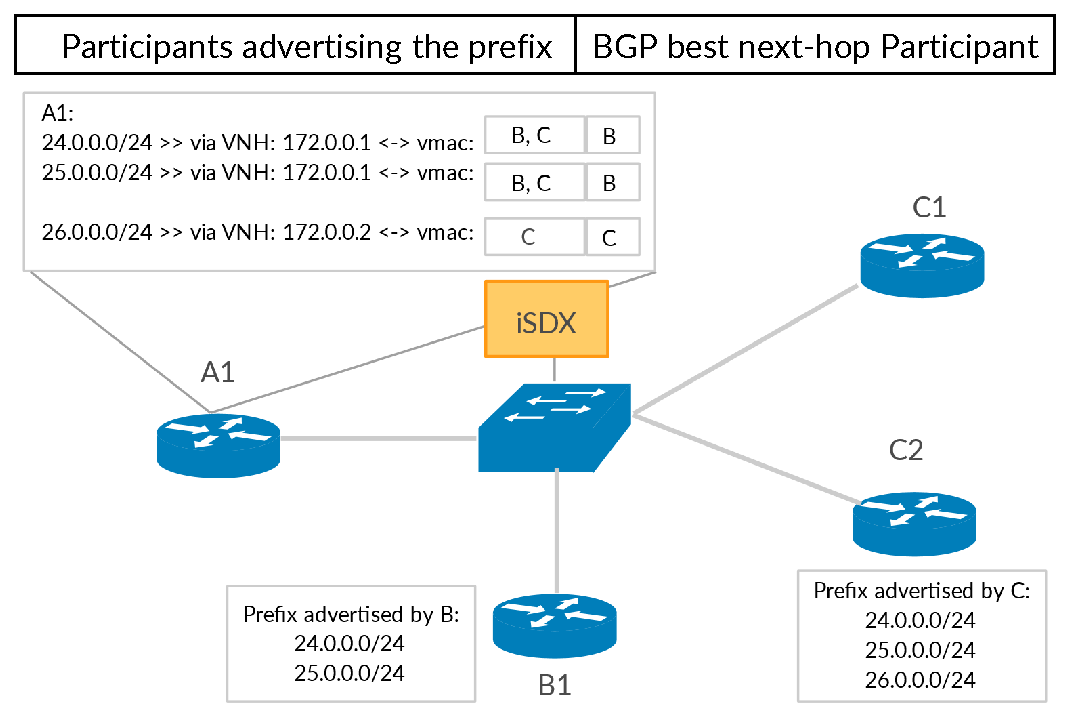
\includegraphics[scale = 0.36]{Figures/bckgrnd_sdx_vmac_cropped.pdf}
\caption{Example of the VMAC at an iSDX connected to three participants}
\label{fig:isdx_vmac}
\end{figure}

\section{\label{chapter2:Swift}Swift}

\rb{adapt the according to how I changed the iSDX part: use for example \emph{(i)} etc}

Swift is a prediction and fast-reroute framework which improves the convergence time of a BGP speaking router upon remote failures. Swifts prediction relies on the fact that the cause of a burst of withdrawals can be predicted before receiving all the withdrawals using the attributes of the already received withdrawals.

In this section, we first show the Swift architecture in \ref{chapter2:Swift:Architecture_SWift}, explain the encoding in \ref{chapter2:Swift:encoding_of_routing_information} and how Swift is able to reduce the convergence time of a router in \ref{chapter2:Swift:BPA}.

\subsection{\label{chapter2:Swift:Architecture_SWift}Architecture}

\begin{figure}[h]
\center
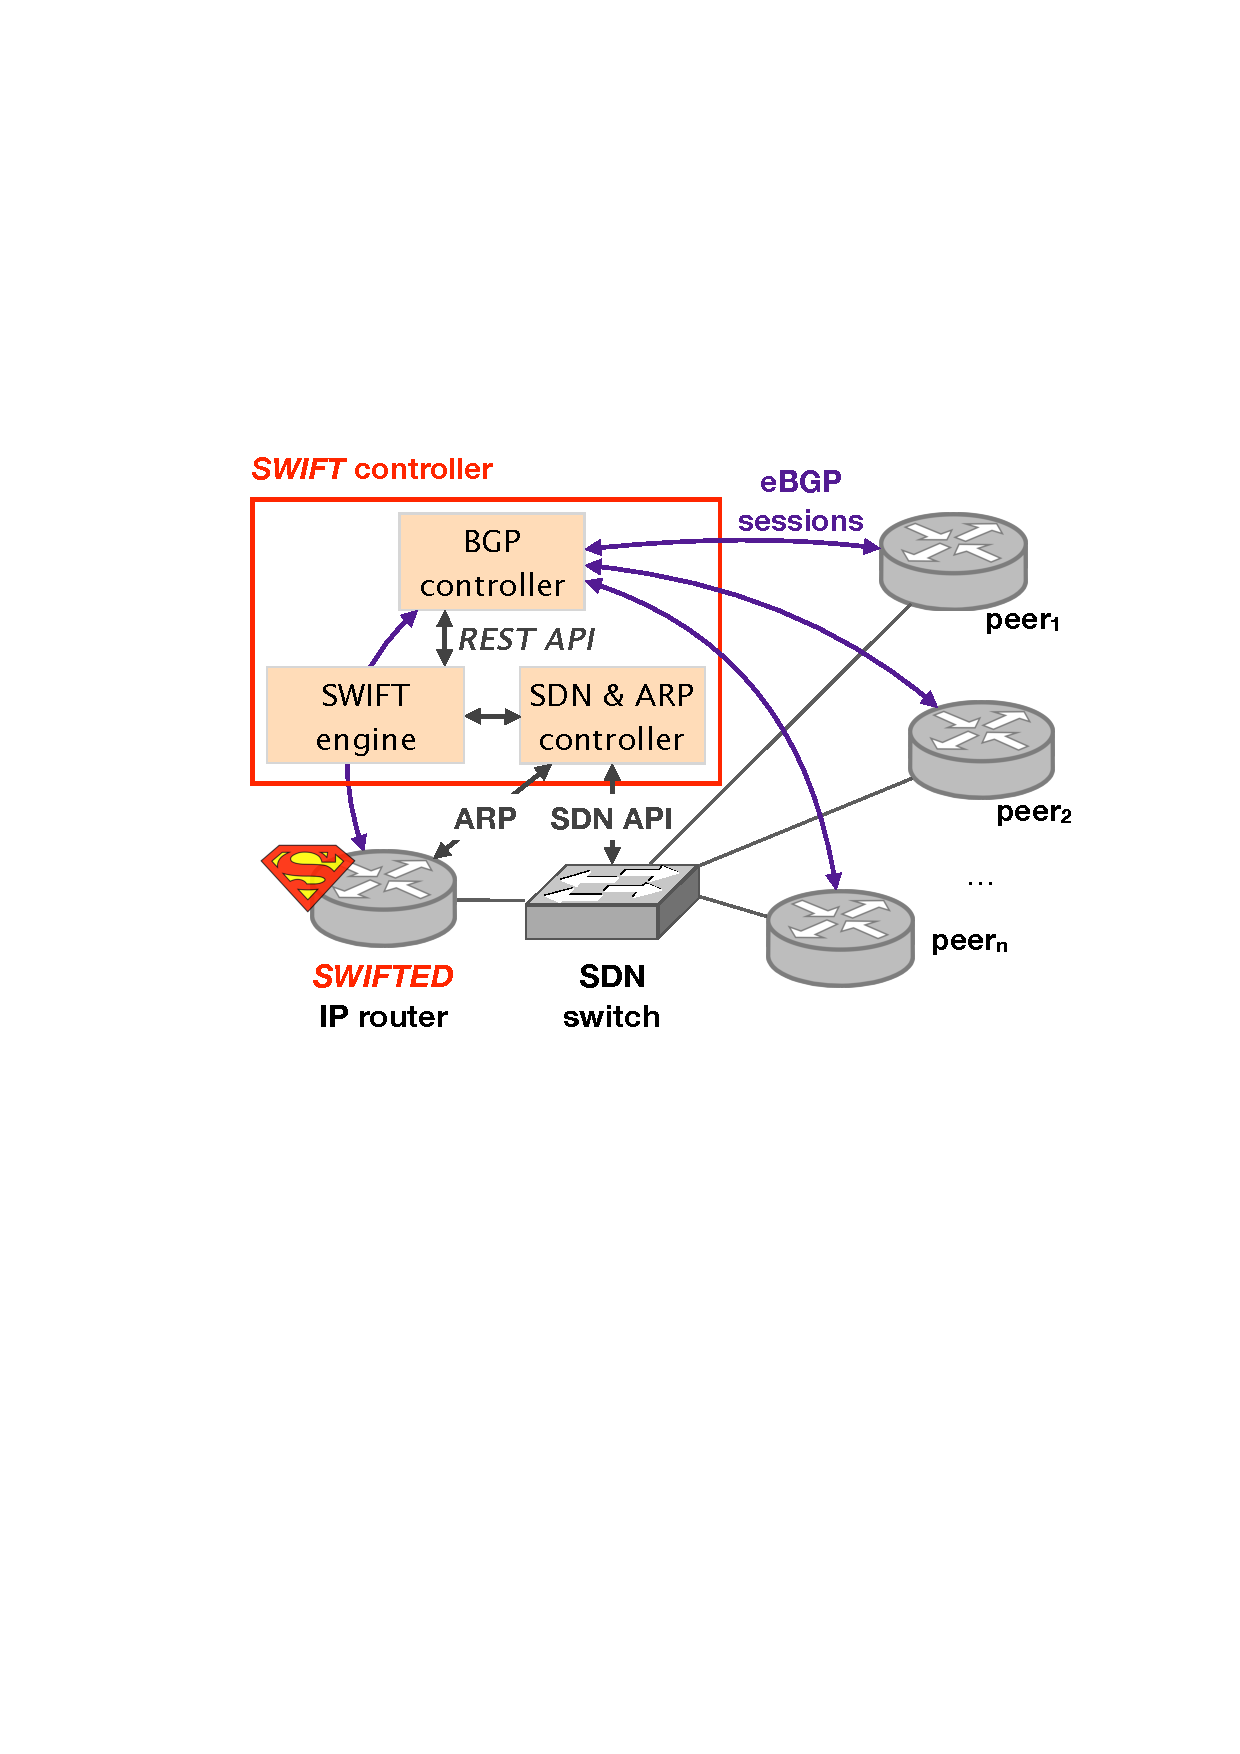
\includegraphics[scale = 0.5]{Figures/bckgrnd_swift_architecture.pdf}
\caption{Example topology of a swifted router}
\end{figure}

Swift uses an SDN switch connected to the swifted router, its neighbors and to the Swift controller. The Swift Controller has three main parts, the  BGP controller, Swift engine and the SDN \& ARP controller. The BGP controller receives BGP updates from the peers of the swifted router. The BGP controller forwards the updates to the Swift engine. The Swift engine consists of two main modules: the burst prediction algorithm and the encoding of routing information. These two modules are the two main features of Swift. The SDN \& ARP controller programs flow rules into the SDN switch and manages ARP requests. \rb{add a sentence in which you say how it is similar to the just shown iSDX architecture and how it differs.}

\rb{I would first have the part about the prediction and then the part about the encoding. You can see as the prediction as the policies of the Swift and then the VMAC. Then, it is easier to understand why you need to have information about backup paths and the AS-links in the VMAC.}

\subsection{\label{chapter2:Swift:encoding_of_routing_information}Encoding of Routing Information}
Swift similarly to the iSDX uses virtual next-hops and the destination mac address to encode the necessary information about the packet and its backup paths.

For every prefix Swift encodes the AS-path up to a certain depth and the backup next-hops for each AS-link on that AS-path. Backup next-hops are neigbhors of the swifted router which also advertise the prefix and their advertised route does not traverse the specific AS-link. This encoding is then mapped to a virtual next-hop. When the swifted router wants to send a packet to any prefix it will use the virtual next-hop assigned by Swift. The virtual next-hop directly maps to the destination MAC address. \\
Figure~\ref{fig:isdx_vmac} shows the swifted router and the VMACs used for the prefixes advertised by the neigbhors.

\paragraph{\label{chapter2:Swift:Swift vmac}Swift VMAC:}

\begin{tabular}{|r|l|}
  \hline 
  backup next-hops for AS-links & AS-path \\
  \hline
\end{tabular}


\begin{figure}[h]
\center
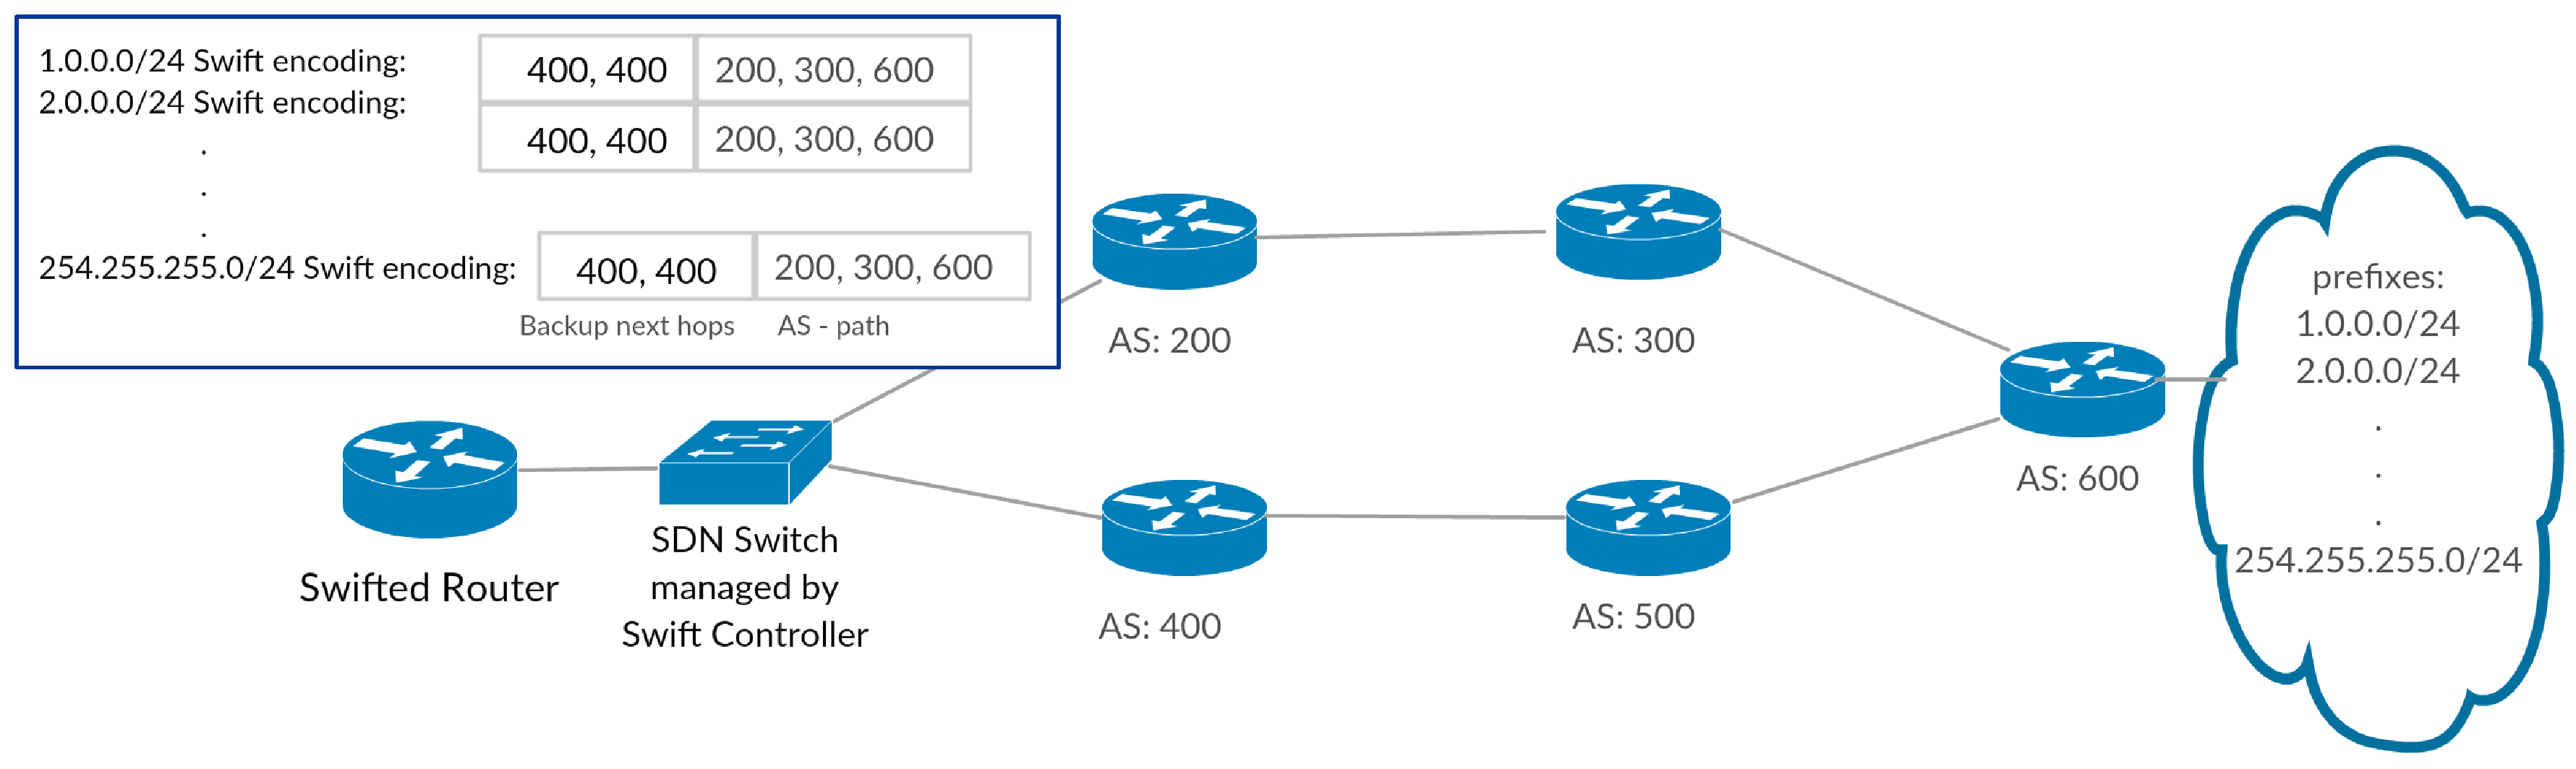
\includegraphics[scale = 0.24]{Figures/bckgrnd_swift_topology.pdf}
\caption{Example of the Swift vmac}
\label{fig:swift_vmac}
\end{figure}


\subsection{\label{chapter2:Swift:BPA}Burst Prediction Algorithm}
\rb{add a sentence describing what is predicted. When is predicted (after receiving x withdraws). Then explain the input, internal state and output as you already do. At the moment, the order is not yet good.}
The burst prediction algorithm takes BGP updates. It uses the updates to build an AS-topology. Once enough withdrawals arrive in a time frame short enough to trigger a burst, the burst prediction algorithm uses the withdrawals and the AS-topology to predict the failed AS-link.

Upon predicting a failed link the Swift Controller pushes Fast Reroute flow rules into the SDN switch matching on the failed AS-link and on the corresponding backup next-hop. In Figure~\ref{fig:isdx_vmac} the burst prediction module has predicted the AS-link 300 600 to be down. So it pushes rules matching on the AS-path 300 600 and the backup next-hop in this case 400.

Every packet that traverses the failed link (has the failed AS-link in it's AS-path encoding) will get rerouted to the backup neighbor.
\begin{figure}[h]
\center
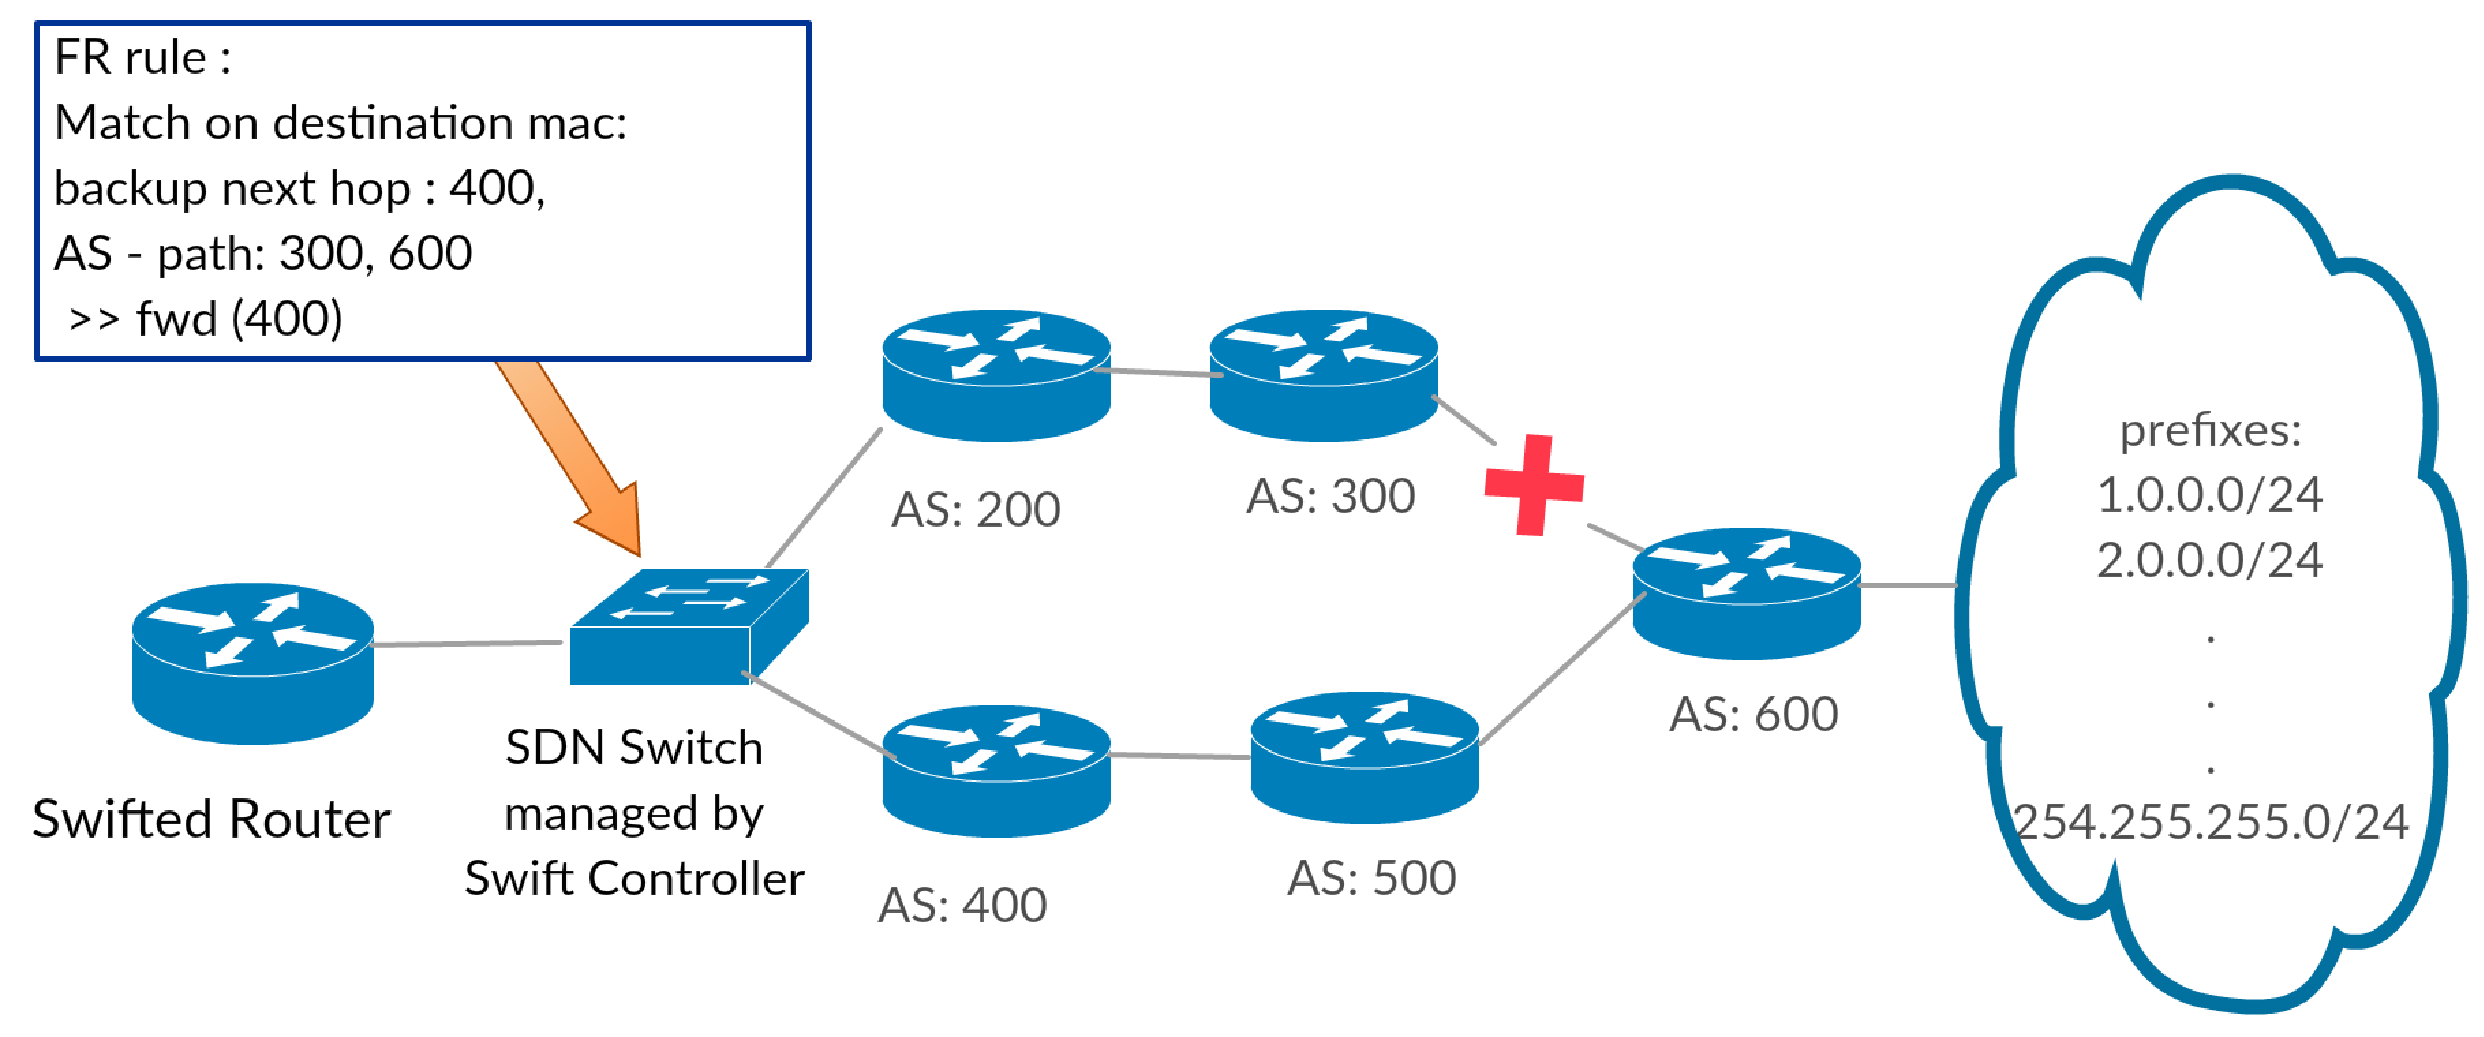
\includegraphics[scale = 0.36]{Figures/bckgrnd_swift_fr.pdf}
\caption{Example of a fast-reroute after BPA predicts the AS link 300 600 to be down}
\label{fig:swift_FR}
\end{figure}

By predicting the failed link and pushing Fast-Reroute rules instead of waiting for all withdrawals to arrive, Swift reduces the convergence time of the swifted router significantly.





